\chapter{Технологическая часть}

В данном разделе будут приведены требования к программному обеспечению, средства реализации и листинги кода.

\section{Требования к программному обеспечению} 
Программа должна предоставлять доступ к функционалу: 
\begin{itemize}[label=---]
	\item перемещение камеры;
	\item изменение интенсивности генерации частиц источником дыма; 
	\item изменение размера и цвета частиц, из которых состоит дым;
	\item вращение, перемещение объектов.
	\item добавление новых объектов на сцену;
	\item изменение интенсивности источника света.
\end{itemize}

\section{Средства реализации}

Для разработки данной программы был выбран язык C\# \cite{sharplang}. Данный выбор обусловлен следующими факторами:
\begin{itemize}[label=---]
	\item язык предоставляет программисту широкие возможности реализации самых разнообразных алгоритмов. Он обладает высокой эффективно-стью и большим набором стандартных классов и процедур;
	\item язык C\# является полностью объектно-ориентированным;
	\item все необходимые инструменты для реализации поставленной задачи находятся в стандартной библиотеке.
\end{itemize}
В качестве среды разработки была выбрана Visual Studio 2022. Среда позволяет работать с .NET Framework, что предоставляет широкий функционал.
\begin{enumerate} 
	\item Мощная библиотека классов. .NET представляет единую для всех поддерживаемых языков библиотеку классов.
	\item Автоматическая сборка мусора, как особенность языка C\# и фреймворка .NET.
	\item JIT-компиляция (Just-In-Time), перекомпиляция исходных файлов во время работы программы.
\end{enumerate}

\section{Реализации алгоритмов}

В листинге \ref{lst:particlemovesystem} приведена реализация алгоритма системы движения частиц.
\captionsetup{justification=raggedright, singlelinecheck=false}
\begin{lstlisting}[label=lst:particlemovesystem,caption=Метод с реализацией ситемы движения частиц.]
public bool Update(double dtime, Vector3 smokerPosition)
{
	float fdtime = (float) dtime;
	Vector3 pos = position - smokerPosition;
	velocity = new(2f * pos.Y * pos.Z, velocity.Y, -2f * pos.X * pos.Y);
	velocity += new Vector3(Random(-3, 3), 0.1f * Random(-1, 1), Random(-3, 3));
	position += velocity * fdtime;
	if (lifeTime > maxLifeTime)
		return true;
	lifeTime += dtime;
	return false;
}
\end{lstlisting}
В листингах \ref{lst:baseraytrace}, \ref{lst:sceneraytrace}, \ref{lst:compraytrace}, 
\ref{lst:shadowraytrace}, \ref{lst:particleraytrace} приведены методы реализующие алгоритм трассировки лучей.
\newpage
\begin{lstlisting}[label=lst:baseraytrace,caption=Основной метод.]
private void RenderPiece(object? param)
{
	int[] p = (int[])(param ?? new[] { 0, 0 });
	int i = p[0];
	int j = p[1];
	Trace t = TraceRay(i - (Cw / 2), -j + (Ch / 2));
	CastShadow(t);
	RenderSmoke(t);
	lbmp.SetPixel(i, j, t.Color);
}
\end{lstlisting}

\begin{lstlisting}[label=lst:sceneraytrace,caption=Метод создания луча взгляда.]
private Trace TraceRay(int x, int y)
{
	Ray r = new(new(x * Vw / Cw, y * Vh / Ch, d), new(0, 0, 0));
	return Composite.TraceRay(r, light);
}
\end{lstlisting}

\begin{lstlisting}[label=lst:compraytrace,caption=Метод нахождения пересечения луча взгляда с объектом сцены Composite.TraceRay.]
public Trace TraceRay(Ray ray, LightSource l)
{
	Trace close = Objects[0].Intersection(ray, l);
	foreach (var obj in Objects)
	{
		Trace t = obj.Intersection(ray, l);
		if (t < close)
		close = t;
	}
	return close;
}
\end{lstlisting}

\begin{lstlisting}[label=lst:shadowraytrace,caption=Метод затенения пересечения луча взгляда с объектом сцены.]
private void CastShadow(Trace trace)
{
	trace.IsShadowed = Composite.CastShadow(trace, light.Position);
	if (!trace.IsShadowed)
	{
		trace.Color = smoke.CastShadow(trace.Point, light.Position, trace.Color);
		smoke.EnableShadowedParticles(trace.Point, light.Position);
	}
	else
	{
		trace.Color = Color.FromArgb((int)(trace.Color.R * 0.3f), (int)(trace.Color.G * 0.3f), (int)(trace.Color.B * 0.3f));
	}
}
\end{lstlisting}

\begin{lstlisting}[label=lst:particleraytrace,caption=Метод отрисовки частиц дыма.]
private void RenderSmoke(Trace trace)
{
	trace.Color = smoke.Intersection(new(0, 0, 0), trace.Point, trace.Color);
}
\end{lstlisting}

\section{Тестирование}
Тестирование выполнено по методологии белого ящика. Полученное изображение \ref{fig:test} является правильным по результатам экспертной оценки.
\begin{figure}[H]
	\centering
	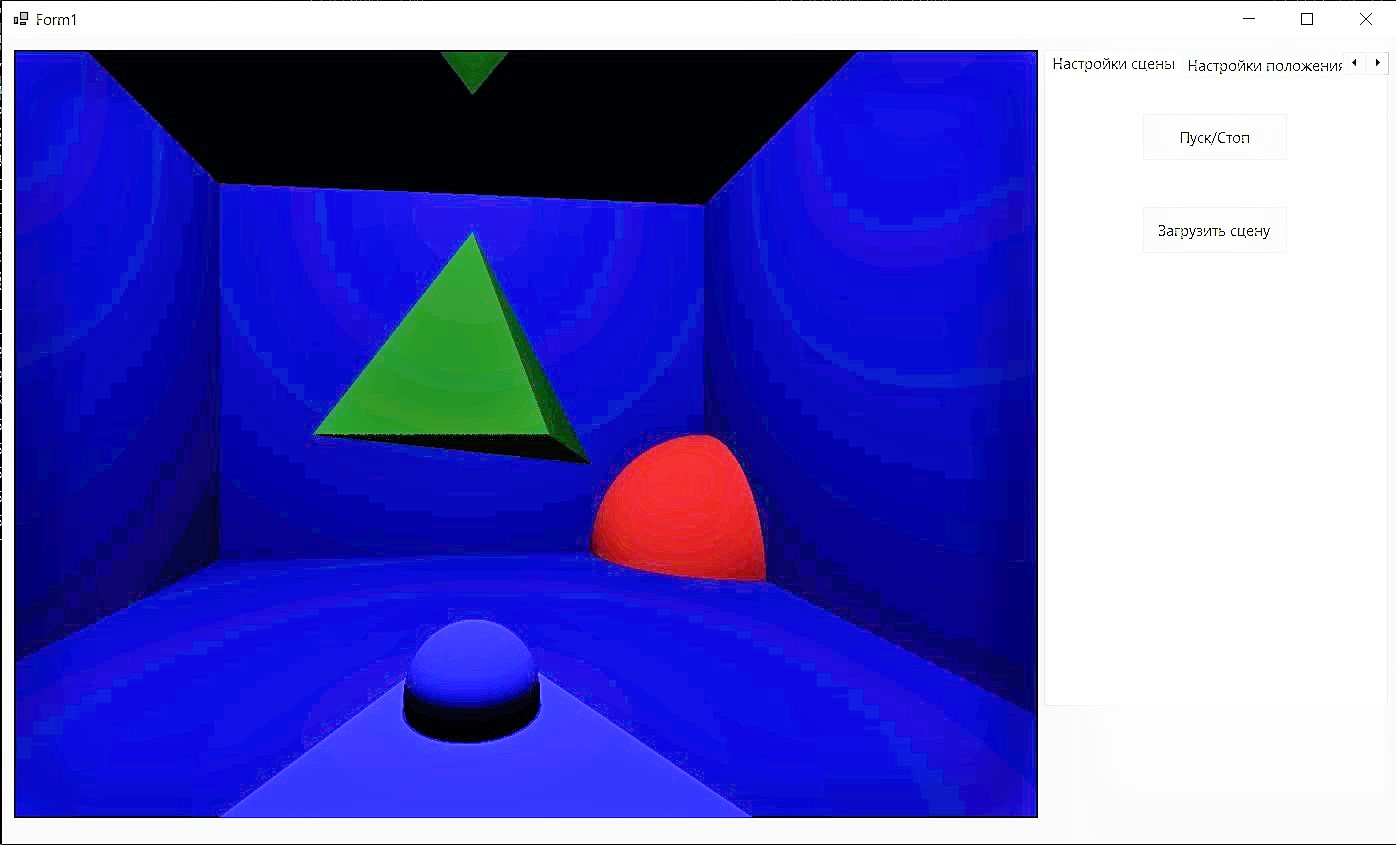
\includegraphics[width=1\linewidth]{inc/img/democlear}
	\caption{Полученное изображение}
	\label{fig:test}
\end{figure}

\section{Демонстрация работы программы}

На рисунках \ref{fig:democlear}, \ref{fig:demosmoke}, \ref{fig:demoblue} представлен результат работы программы 
\begin{figure}[H]
	\centering
	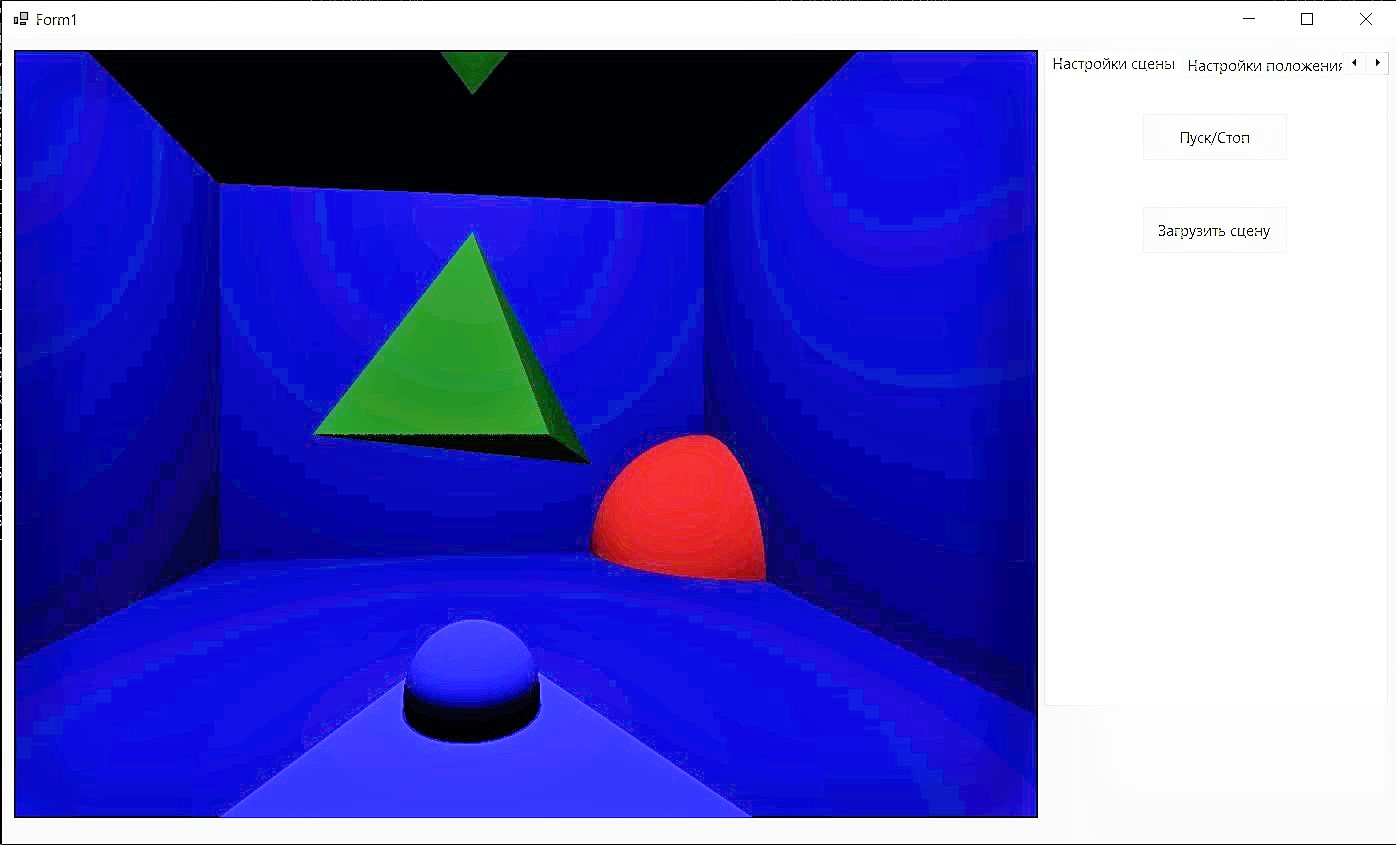
\includegraphics[width=1\linewidth]{inc/img/democlear}
	\caption{Результат работы программы в комнате без дыма}
	\label{fig:democlear}
\end{figure}
\begin{figure}[H]
	\centering
	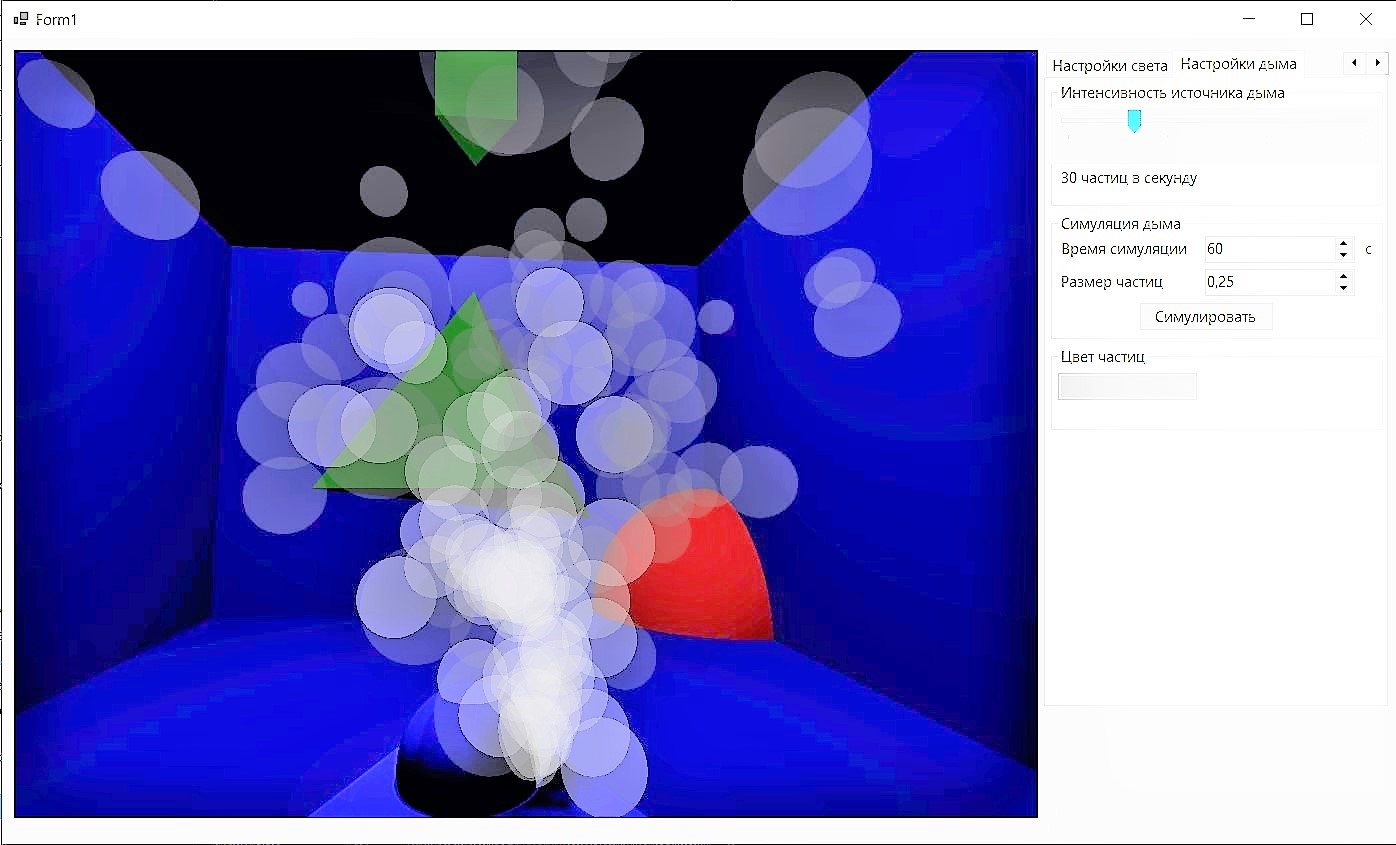
\includegraphics[width=1\linewidth]{inc/img/demosmoke}
	\caption{Результат работы программы с дымом}
	\label{fig:demosmoke}
\end{figure}
\begin{figure}[H]
	\centering
	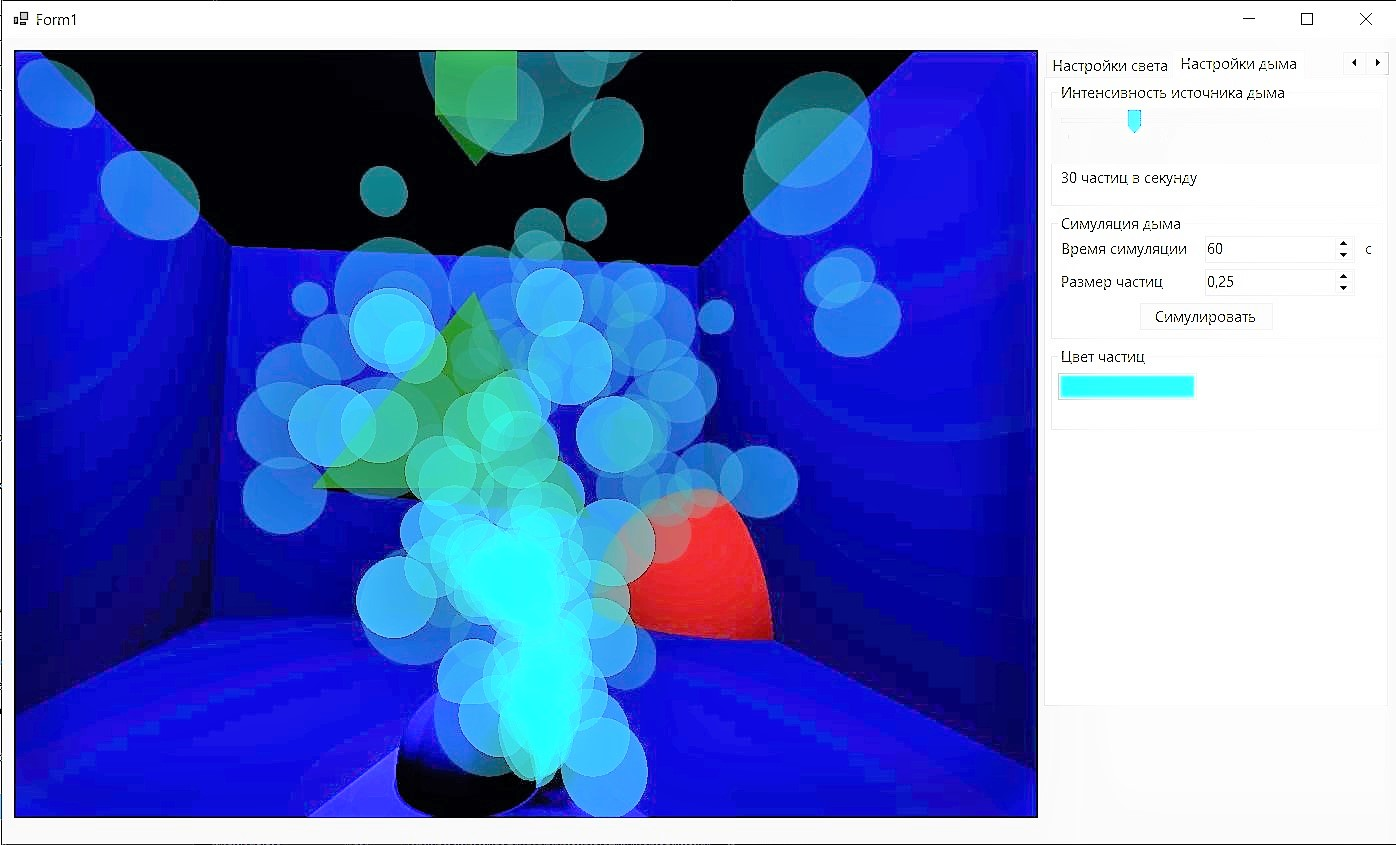
\includegraphics[width=1\linewidth]{inc/img/demoblue}
	\caption{Результат работы программы с голубым дымом}
	\label{fig:demoblue}
\end{figure}

\section*{Вывод}

В данном разделе были рассмотрены средства реализации программного обеспечения и листинги исходных кодов программного обеспечения, разработанные на основе алгоритмов, изложенных в конструкторской части., а также проведено тестирование.
